%% ------------------------------------------------------------------------- %%
\chapter{Introdução} %Nome do capítulo.
\setcounter{page}{29}
\label{cap:intro} 
\epigraph{"Tradicionalmente a notação musical é vista como um código através do qual sons, ideias musicais ou indicações para execução musical são registrados sob forma escrita."}{Edson S. Zampronha.\cite{Zampronha} \\}


Representar estruturas e artifícios musicais através das características do som discretizado
é a proposta deste trabalho. Os resultados são relações matemáticas e suas implementações computacionais. Uma descrição teórica está no capítulo~\ref{cap:resultados} e o conjunto de \emph{scripts} disponibilizados no Apêndice~\ref{cap:codigoProc} e online.\cite{MASSA} A \emph{toolbox} resultante recebeu o nome \massa\ (música e áudio em sequências e séries amostrais) e foi utilizada para fazer pequenas peças e montagens focadas nos princípios expostos. O Apêndice~\ref{cap:codigoPecas} possui uma relação destas montagens assim como o diretório \emph{exemplos\_de\_uso} da \massa.

    \section{Som em áudio digital}\label{sec:audio}

O som é uma onda mecânica longitudinal de pressão. A banda de frequências compreendida entre $20Hz$ e $20 kHz$ é apreciada pelo aparelho auditivo humano com variações dependentes da pessoa, das condições climáticas e do som em si.
 Considerada a velocidade do som no ar $\approx 343.2\,m/s$,
estes limites correspondem respectivamente aos comprimentos de onda $\frac{343.2}{20} = 17.16\,m$ e $\frac{343.2}{20000}=17.16\,mm$.\cite{Roederer}


A percepção humana do som envolve captações pelos ossos, estômago e orelha, funções de transferência da cabeça e dorso e processamento pelo sistema nervoso. Além disso, o ouvido é um órgão dedicado à captura destas ondas. Seu funcionamento decompõe o som em seu espectro senoidal e passa para o sistema nervoso.\cite{Roederer} Estas componentes senoidais são cruciais para os fenômenos musicais, como se pode observar tanto na composição dos sons de interesse para a música quanto nas afinações e escalas.\cite{floEsp} A subseção~\ref{sec:notaDisc} expõe a presença de senoides no som discretizado e caracteriza a nota musical básica.

A representação do som é o áudio\footnote{Os termos
som e áudio são muitas vezes usados de forma intercambiável.\cite{Everest}} e este pode provir da captura do som por microfones ou da síntese. Muitas vezes, o áudio digital é especificado através de protocolos que facilitam o armazenamento e transferência dos arquivos. A representação digital do som pode consistir em amostras igualmente espaçadas no tempo e cujas amplitudes individuais são registradas com um mesmo número de \emph{bits}. Estas amostras separadas por intervalos regulares $\lambda_a$ constituem a forma padrão de representação do som em tempo discreto, chamada de modulação por código de pulsos (PCM do inglês \emph{Pulse Code Modulation}).
Um som digital PCM é caracterizado pela frequência de amostragem $f_a=\frac{1}{\lambda_a}$, também chamada de taxa de amostragem, e a profundidade de \emph{bit} que é o número de \emph{bits} utilizados para representar a amplitude de cada amostra. A figura~\ref{fig:PCM} exibe $25$ amostras de um áudio PCM com $4$ \emph{bits} cada. Os $2^4=16$ grados para a amplitude de cada amostra junto ao espaçamento regular $\lambda_a$ introduzem um erro de quantização. O ruído causado por estes erros diminuem com a diminuição destes espaçamentos.\cite{audioMedia} 


\begin{figure}[h!]
    \centering
        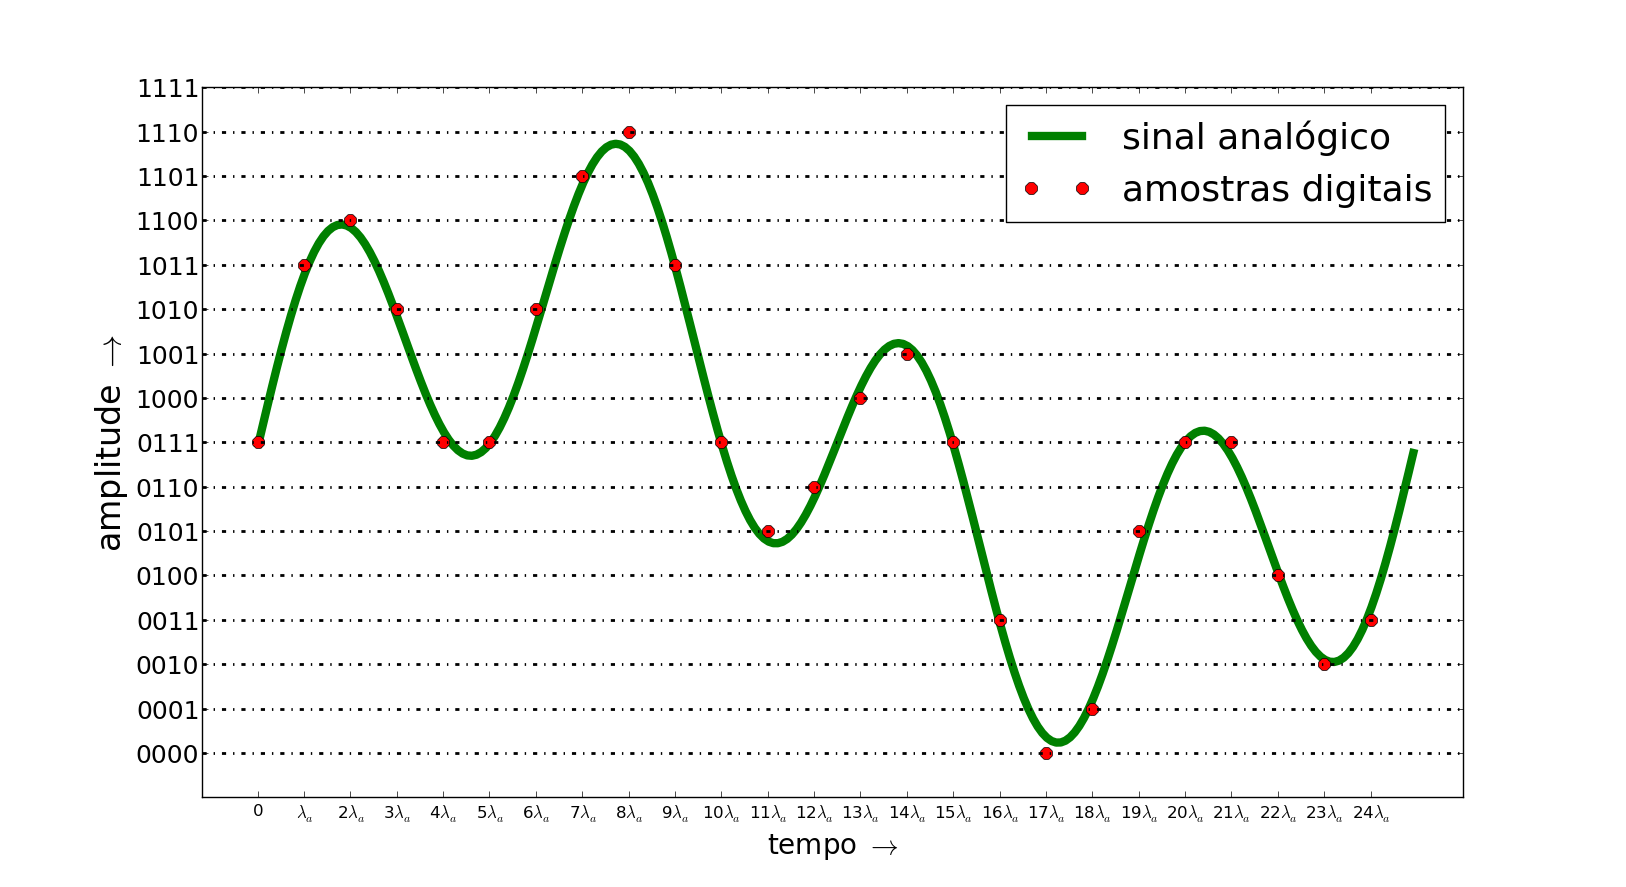
\includegraphics[width=\textwidth]{figuras/pcm}
        \caption{Som digital em modulação por código de pulsos (PCM): 25 amostras representadas por 4 bits cada uma.}
        \label{fig:PCM}
\end{figure}

Pelo teorema de Nyquist, constata-se que a metade da frequência de amostragem é a frequência máxima do sinal. Assim, para apreender as frequências audíveis, é necessária uma taxa de amostragem que seja ao menos o dobro da frequência mais aguda $f_a \geq 2\times 20kHz=40kHz$. Este raciocínio está na base da utilização das frequências de amostragem $f_a=44.1kHz$ e $f_a=48kHz$, ambas padrão em \emph{Compact Disks} (CDs) e em sistemas de Rádio e TV, respectivamente.\cite{audioMedia}


    \section{Arte sonora e teoria musical}

A música é definida como a arte manifesta pelos sons e silêncios. Para um ouvinte comum - e boa parte dos especialistas - uma 'música que seja música' pressupõe também uma métrica rítmica e organizações de alturas que formem melodias e harmonias como explicadas na seção~\ref{notasMusica}. A música do século XX ampliou esta concepção tradicional de música. Isso ocorreu na música de concerto, especialmente nas correntes concreta, eletrônica e eletroacústica. Já na década de 90 era evidente que também a música popular, especialmente as músicas eletrônicas de dança, tinham incorporado sons sem altura definida e organizações temporais fora de métricas simples. Mesmo assim, a nota permanece paradigmática como 'unidade fundamental' das estruturas musicais e, na prática, pode se desdobrar em sons que contemplam estes desenvolvimentos recentes. A nota musical e sua expansão são abordadas na seção~\ref{varInternas}.\cite{Wisnick,Webern,Lerdahl,Cook}

A teoria musical engloba assuntos tão diversos quanto psico-acústica, manifestações culturais e formalismos. O texto do capítulo~\ref{cap:resultados} aborda estes assuntos mediante necessidade e assinala complementos externos.\cite{Zamacois,Schoenberg,microsound}



    \section{Implementação computacional}
Os resultados apresentados desta dissertação incluem \emph{scripts}, i.e. pequenos programas para melhor disponibilidade e validação das tecnologias, que constituem a caixa de ferramentas \massa. Este conjunto de códigos está disponibilizado em domínio público através de repositórios Git públicos.\cite{gitBook}
Os \emph{scripts} estão em Python e fazem uso das bibliotecas externas Numpy e Scikits/Audiolab que realizam chamadas à linguagem Fortran para maior eficiência computacional. Parte deste código foi transcrito para JavaScript e Python nativos com facilidade, o que aponta para um uso destas contribuições em navegadores como o Firefox e o Chromium.\cite{numpy,audiolab,tutPython,python}

Estas tecnologias são todas abertas, i.e. estão publicadas em licenças que permitem o uso, cópia, distribuição e utilização de quaisquer partes para estudo e geração de produtos derivados. Desta forma, o trabalho aqui descrito está disponível e facilita os processos de co-autoria\footnote{A comunidade e movimento chamada \emph{'Open Source'} entende a publicação de código computacional (e outras tecnologias) em licenças abertas como uma vantagem pragmática que facilita o desenvolvimento de \emph{software} e apresenta vantagens pedagógicas e mercadológicas. A comunidade e movimento chamada \emph{'Free Software'} engloba este entendimento, mas adiciona a abordagem filosófica da liberdade e compartilhamento, dando ênfase a isso. Ambas as correntes reforçam o entendimento de que o código computacional é o 'bem mais precioso produzido atualmente' pois consiste em tecnologia condensada, reativa (executa, processa ou gera resultados), modular (partes são copiadas e reutilizadas eficientemente) e replicada sem custo adicional (a cópia de texto tem custo baixíssimo).\cite{Raymond,Lessig}}.

    \section{Objetivos}
   \label{sec:objetivos}
O objetivo principal desta dissertação é apresentar de forma unificada relações entre elementos básicos da música e as sequências amostrais do áudio PCM. O capítulo seguinte é um texto conciso em que os elementos musicais são apresentados junto às amostras temporais resultantes. Para validação e compartilhamento, as implementações em código computacional destas relações e de pequenas peças musicais\footnote{Ou, de forma menos pretenciosa, montagens musicais, sequências musicais.} foram reunidas em uma \emph{toolbox} chamada \massa\ e disponibilizadas online e parcialmente nos Apêndices~\ref{cap:codigoProc} e~\ref{cap:codigoPecas}. 

Dos objetivos secundários, destaca-se a difusão da compreensão do código computacional através de práticas lúdicas, no caso a música. Outro objetivo considerado é a apresentação de um arcabouço de síntese sonora e musical com controle amostral, para o qual há potenciais usos em experimentos psico-acústicos e síntese em alta definição (\emph{hi-fi}). Também é considerada a apresentação destes conteúdos de forma didática, quase um tutorial, o que possibilita compreensão e uso facilitados. Esta exposição amistosa faz-se significativa pois os assuntos tratados são de reconhecida complexidade: processamento de sinais, música, psico-acústica, para citar somente alguns exemplos. Deste ponto de vista pedagógico, também se presta a apresentação destes resultados na forma de hipertexto, em que cada \emph{script} e exemplo sonoro/musical seja acessível junto ao material teórico.
  
